\section{AUV Modelling}
\label{sec:model}


The equations of motion for the rigid body are described in a body-fixed coordinate system in the \ac{NED} frame (See Fig. \ref{fig:rov}) \cite{fossen}. Neglecting roll and pitch motion due to the restoring moment action significantly simplifies the equations of motion. This assumption, as adopted in \cite{shen2018path, heshmati2019robust}, enables more focus on the dominant dynamics of the system, which can be written as follows:

\begin{figure}[b!]
	\centering	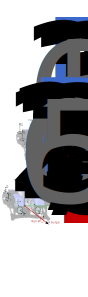
\includegraphics[width=0.7\linewidth]{figures/Introduction/brov.pdf}
	\caption{\ac{AUV} free body diagram and reference frames \cite{unav}.}
	\label{fig:rov}
\end{figure}


\begin{align}
\dot{x} &= \cos(\psi) u - \sin(\psi)  v \label{eq:xdot}\\
\dot{y} &= \sin(\psi)  u + \cos(\psi)  v \label{eq:ydot}\\
\dot{z} &= w \label{eq:zdot}
\end{align}
\begin{align}
(m - X_{\dot{u}})\dot{u} &= X + (m  v + Y_{\dot{v}}  v)  r \nonumber \\
&\quad + (X_u + X_{uc}  |u| )  u + \Delta_{x} \label{eq:udot}\\
(m - Y_{\dot{v}})\dot{v} &= Y - (m  u + X_{\dot{u}}  u)  r \nonumber \\
&\quad + (Y_v + Y_{vc}  |v|)  v + \Delta_{y} \label{eq:vdot}\\
(m - Z_{\dot{w}}) \dot{w} &= Z + (Z_w + Z_{wc}  |w|)w \nonumber \\
&\quad + m  g - V_{sub} \rho_{water}  + \Delta_{z}\label{eq:wdot}\\
\dot{\psi} &= r \label{eq:psidot}\\
(I_{zz} - N_{\dot{r}}) \dot{r} &= M_z - (m  v - Y_{\dot{v}}  v)  u \nonumber \\
&\quad - (X_{\dot{u}}  u - m  u)  v  \nonumber \\
&\quad + (N_r + N_{rc}  |r|)  r + \Delta_{M_z} \label{eq:rdot}
\end{align}

In the equations above, the translational positions $x$, $y$, and $z$ are specified within the earth-fixed frame $\mathcal{F}_E$. The translational velocities $u$, $v$, and $w$ are represented in the body frame $\mathcal{F}_B$, whereas $r$ denotes the rotational velocity about the z-direction. Translational velocities in $\mathcal{F}_E$ can be obtained by rotating the body velocities with an angle $\psi$ about the heave direction. The vehicle's mass is denoted by $m$, the angular moment of inertia about the z-axis is denoted as $I_{zz}$, $g$ describes the gravitational constant, $\rho_{water}$ is the water density, and $V_{sub}$ denotes the total submerged volume. $X$, $Y$, and $Z$ denote applied wrenches by actuators acting on the \ac{AUV} body in $\mathcal{F}_B$, while $M_z$ represents the externally applied moment about the z-axis. Here, $\mathbf{\Delta}  \in \mathbb{R}^{4}$ given by [$\Delta_{x}$, $\Delta_{y}$, $\Delta_{z}$ $\Delta_{M_z}$] are the external disturbances affecting the \ac{AUV} body in the body frame. This term accounts for the lumped unmodeled disturbances arising from currents, tether, and other effects.


The parameters $X_{\dot{u}}$, $Y_{\dot{v}}$, $Z_{\dot{w}}$, and $N_{\dot{r}}$ represent added mass parameters. $X_{u}$, $Y_{v}$, $Z_{w}$, and $N_{r}$, as well as $X_{uc}$, $Y_{vc}$, $Z_{wc}$, and $N_{rc}$, denotes linear and quadratic drag coefficients about the surge, sway, heave, and yaw directions, respectively. The parameters for the BlueROV2 heavy model, used for both simulation and controller model, are provided in Table \ref{tab:brovparams}. The equations of motion can also be rewritten in state-space form:



\begin{table*}[t]
\caption{BlueROV2 heavy parameters}
\centering
\normalsize
\setlength{\tabcolsep}{4pt} % Adjust column spacing if needed
\renewcommand{\arraystretch}{1.5} % Adjust row height (1.0 is normal}
\begin{tabular}{|c|c|c|c|c|c|c|c|c|c|c|c|c|c|c|}
\hline
$X_{\dot{u}}$ & $Y_{\dot{v}}$ & $Z_{\dot{w}}$ & $N_{\dot{r}}$ & 
$X_{u}$ & $Y_{v}$ & $Z_{w}$ & $N_{r}$ & $X_{uc}$ & $Y_{vc}$ & $Z_{wc}$ & $N_{rc}$ & $m$ & $V_{sub}$ & $I_{zz}$ \\ \hline
-2.6 & -18.5 & -13.3 & -0.28 & 
-0.09 & -0.26 & -0.19 & -4.64 & -34.9 & -103.25 & -74.2 & -0.43 & 11.4 & 115 & 0.24 \\ \hline
\end{tabular}

\label{tab:brovparams}
\vspace{-0.3cm}
\end{table*}

%
\begin{align} \label{eq:model_eqs}
    \dot{\mathbf{x}} = \mathtt{f}(\mathbf{x}_k,\mathbf{u}_k, \mathbf{\Delta}),  \quad
   % \mathtt{z}_k = \mathtt{h}(\mathtt{x}_k,\mathtt{u}_k),
\end{align}
%
 The vectors $\mathbf{x} \in \mathbb{R}^{8}$ and $\mathbf{u} \in \mathbb{R}^{4}$  denote the state and control vectors, respectively
%
\begin{align}
\label{eq:state_control} 
    \mathbf{x} &= [x,y,z,u,v,w, \psi, r]^T, \quad  \\
    \label{eq:control} 
    \mathbf{u} &= [X,Y,Z,M_z]^T.
\end{align}
%
The state transition function is represented by $\mathtt{f}(\cdot,\cdot, \cdot)$: $\mathbb{R}^{8} \times \mathbb{R}^{4} \times 
 \mathbb{R}^{4} \rightarrow \mathbb{R}^{8}$.

 
%\begin{align} \label{eq:state_trans}
%   \textcolor{red}{ \mathtt{f}(\mathbf{x}_k,\mathbf{u}_k) = %\mathbf{x}_k + \Delta t \hspace{0.1cm}  \dot{\mathbf{x}_k}}
   % \mathtt{z}_k = \mathtt{h}(\mathtt{x}_k,\mathtt{u}_k),
%\end{align}.

%\textcolor{red}{where $\Delta t$ is the time step.}

















 



 

